% UNLP 2026 Shared Task System Description Paper
% ACL Short Paper (4 pages content + unlimited references)
% Updated: 2026-04-07
\documentclass[11pt]{article}
\usepackage[hyperref]{acl2023}
\usepackage{times}
\usepackage{latexsym}
\usepackage{booktabs}
\usepackage{graphicx}
\usepackage{amsmath}
\usepackage{multirow}
\usepackage[utf8]{inputenc}
\usepackage[T1]{fontenc}
\usepackage[english]{babel}
\usepackage{pgfplots}
\pgfplotsset{compat=1.17}
\usepackage{tikz}
\emergencystretch=2em

\title{When Local Wins Fail to Generalize: \\
PFW at UNLP 2026 Ukrainian Document QA}

\author{
  Taleef Tamsal \\
  Purdue University \\
  {\small\texttt{tamst01@purdue.edu}}
}

\date{}

\begin{document}
\maketitle

\begin{abstract}
We describe our system for the UNLP 2026 Shared Task on Ukrainian document question answering~\cite{unlp2026task}, in which systems must answer 6-option multiple-choice questions from a corpus of domain-specific PDFs while localizing the answer to the correct document and page (metric: $0.5a + 0.25d + 0.25p$).
Our final submission achieves a \textbf{private score of 0.8722 (rank 7 of 15)}, using BGE-M3 dense retrieval~\cite{chen2024bge}, a Qwen3-0.6B~\cite{qwen3_2025} cross-encoder page reranker, and MamayLM-Gemma-3-12B~\cite{mamaylm2025} with 3-pass voting.
Post-competition analysis reveals a consistent \textit{local-vs-Kaggle generalization gap}: every offline improvement (up to $+$0.018 composite) regressed on the private leaderboard, while our conservative baseline proved most robust.
A no-retrieval closed-book baseline scores 66.8\% answer accuracy vs.\ 88.5\% for our system, confirming retrieval-enabled inference provides $+$21.7 pp over the retrieval-disabled (closed-book) baseline. Key negative results: BM25+BGE-M3 fusion ($-$27 pp Doc@1), ColSmol visual retrieval (Doc@1 $\approx$ 0), and chain-of-thought prompting (14.3\%, near-random).
\end{abstract}

\section{Introduction}

The UNLP 2026 Shared Task~\cite{unlp2026task} requires teams to answer 6-option Ukrainian MCQs from $\sim$240 domain-specific PDF documents (estimated test corpus; the development set used here contains 41 PDFs), while localizing the answer to the correct document and page.
The composite metric is:
\begin{equation}
  S = 0.5\,a_i + 0.25\,d_i + 0.25\,p_i
  \label{eq:metric}
\end{equation}
where $a_i$, $d_i$ are answer and document correctness, and $p_i = \max(0,\,1 - |p_\text{pred}-p_\text{true}|/N)$ is page proximity ($N$ = total pages in the predicted document). Note that $N$ is the page count of the \emph{predicted} document: a wrong-document prediction changes the denominator, so a shorter predicted document imposes a harsher per-page penalty, creating a coupling between document and page accuracy.

The competition ran on Kaggle (T4$\times$2, 9-hour limit, no internet) and comprised 15 teams; the winning team scored 0.9598 privately.
Our central finding is that \textit{conservatism beats local optimization under hidden domain shift}: despite over a dozen offline ablations, no local improvement transferred reliably to Kaggle.
This paper contributes a complete description of v7, offline ablations covering retrieval, reranking, and prompting, and a formalized post-competition analysis of failure modes and risk signals (\S\ref{sec:gap}).

\section{Task and Data}

The development set contains 461 questions spanning two visible domains: Domain 1 (sports regulations, 11 documents, 865 pages, avg.\ 78.6 pages/doc) and Domain 2 (medical guidelines, 30 documents, 256 pages, avg.\ 8.5 pages/doc). Answer labels are approximately uniform across options A--F. Text extraction via PyMuPDF takes $\sim$4s for all 1,121 pages; 16 pages in Domain 2 have $<$50 characters (scanned content).

The private test set contains a \textit{hidden third domain} not present in development, which we identify as the primary driver of the local-vs-Kaggle gap (\S\ref{sec:gap}).

We use three offline evaluation protocols: \textbf{full-dev} (all 461 questions), \textbf{grouped CV} (5-fold, stratified by document identity to prevent document-level memorization from inflating fold scores), and \textbf{lockbox} (fixed 20\% held-out document partition). Promotion to Kaggle submission requires passing all three gates.

\section{Related Work}
\label{sec:related}

\paragraph{Multilingual Dense Retrieval.}
Dense retrieval for open-domain QA~\cite{lewis2020retrieval} has been extended to multilingual settings via contrastive pre-training~\cite{izacard2022unsupervised} and multilingual benchmarks such as MIRACL~\cite{zhang2023miracl}. BGE-M3~\cite{chen2024bge} advances this with multi-functionality and multi-granularity retrieval; its strong Ukrainian performance (\S\ref{sec:retrieval}) motivates our choice over BM25 or visual methods.

\paragraph{RAG for Document QA.}
Multi-page document understanding~\cite{cho2024m3docrag} and dense-retrieval MCQ pipelines share the retrieve-then-read paradigm~\cite{lewis2020retrieval}. Visual retrieval models (ColPali~\cite{faysse2024colpali}) show promise on Latin-script layouts; our Ukrainian Cyrillic corpus exposes their limitations (\S\ref{sec:retrieval}).

\paragraph{Domain Shift in NLP.}
Pre-trained models remain brittle under distribution shift~\cite{hendrycks2020pretrained}. Shared task evaluations routinely reveal local-vs-held-out gaps; our contribution is formalized risk signals (\S\ref{sec:gap}) for predicting such failures before submission.

\section{System Description (v7)}
\label{sec:system}

Our competition system follows four stages.

\paragraph{Stage 1: Text Extraction.}
PyMuPDF extracts page-level plain text; no OCR fallback.

\paragraph{Stage 2: Dense Retrieval.}
We embed all pages and queries using BGE-M3~\cite{chen2024bge} in FP16, stored in FAISS~\cite{johnson2019billion} \texttt{IndexFlatIP}. The query is question text only — adding answer options hurts Doc@1 by 7.6 pp. We retrieve top-10 pages and forward top-3 scoring documents.

\paragraph{Stage 3: Page-Level Reranking.}
A Qwen3-0.6B~\cite{qwen3_2025} cross-encoder rescores all pages within each candidate document (\texttt{max\_length}=2048, query = question + all six options). The top-1 page per document determines the final document; page reranking improves page recall@1 from 0.471 to 0.538 ($+$6.7 pp).

\paragraph{Stage 4: MCQ Answer Generation.}
MamayLM-Gemma-3-12B-IT~\cite{mamaylm2025}, quantized to Q4\_K\_M (6.8\,GB), is served via \texttt{llama.cpp}~\cite{llamacpp} with greedy decoding ($T=0$). The prompt concatenates the top-2 pages of the chosen document, the question, and six answer options, ending with the directive ``Answer (letter only):'' in Ukrainian; no chat template is applied (an early ablation showed $-$0.028 on fold-1; direct prompting outperforms template-wrapped inference in-distribution). We apply 3-pass majority voting; unanimous votes (77.2\% of questions) achieve 90.2\% answer accuracy vs.\ 83.7\% for majority-only votes ($+$6.5 pp), confirming voting confidence as a proxy for difficulty.

\section{Retrieval Experiments}
\label{sec:retrieval}

\begin{table}[t]
\centering
\resizebox{\columnwidth}{!}{%
\begin{tabular}{lcccc}
\toprule
\textbf{System} & \textbf{Doc@1}\textsuperscript{$\dagger$} & \textbf{Doc@10} & \textbf{Pg@1} & \textbf{Pg@10} \\
\midrule
Random & 0.056 & --- & --- & --- \\
BM25 & 0.458 & 0.781 & 0.219 & 0.547 \\
\textbf{BGE-M3} & \textbf{0.933} & \textbf{0.994} & \textbf{0.482} & \textbf{0.796} \\
BM25+M3 (RRF) & 0.659 & 0.991 & 0.343 & 0.831 \\
ColSmol-500M & 0.039 & 0.074 & 0.000 & 0.000 \\
M3+ColSmol (RRF) & 0.928 & --- & 0.479 & --- \\
\bottomrule
\end{tabular}%
}
\caption{Retrieval on full dev ($N$=461). \textbf{Bold} = best. \textsuperscript{$\dagger$}Doc@$k$: fraction of questions for which the true document is in the top-$k$ retrieved; Pg@$k$: same for the true page.}
\label{tab:retrieval}
\end{table}

BGE-M3 achieves Doc@1 = 0.933, dramatically outperforming BM25 (0.458). Hybrid fusion (RRF, $k$=60) drops Doc@1 to 0.659 ($-$27.4 pp): BM25's weak Ukrainian performance introduces noise that corrupts BGE-M3's strong top-1 results, contrasting with English benchmarks where hybrid retrieval helps \cite{luan2021sparse,robertson2009probabilistic}.

ColSmol-500M~\cite{faysse2024colpali} achieves Doc@1 = 0.039. FP16 normalization produces NaN query embeddings for Ukrainian Cyrillic input; correcting this yields Doc@1 = 0.039, consistent with ColPali's training on Latin-script visual document layouts rather than Cyrillic OCR text.

\section{Main Results}
\label{sec:results}

\begin{table}[t]
\centering
\resizebox{\columnwidth}{!}{%
\begin{tabular}{lccccr}
\toprule
\textbf{System} & \textbf{Ans.} & \textbf{Doc} & \textbf{Page} & \textbf{Comp.} & \textbf{Rerank} \\
\midrule
Closed-book ($k$=0) & .668 & --- & --- & .749 & --- \\
\midrule
v7 (0.6B reranker) & .885 & .889 & .794 & .8634 & 624s \\
\quad+ Fair 4B reranker & .889 & .937 & .831 & .8866 & 2131s \\
\bottomrule
\end{tabular}%
}
\caption{Full-dev results ($N$=461). Closed-book: retrieval disabled. Fair 4B vs.\ v7: $\Delta{=}{+}0.023$, bootstrap CI $[{+}0.006,{+}0.041]$. Rerank column shows reranking stage wall time on A30.}
\label{tab:main}
\end{table}

Table~\ref{tab:main} shows full-dev results. The closed-book baseline achieves 66.8\% answer accuracy and 74.9\% composite, confirming retrieval contributes $+$21.7 pp to answer accuracy and $+$11.5 pp to composite.

The \textbf{fair 4B reranker} replaces Qwen3-0.6B with Qwen3-4B~\cite{qwen3_2025} at the same \texttt{max\_length}=2048, improving composite by $+$0.023 (bootstrap CI $[{+}0.006,{+}0.041]$, entirely positive; driven by document accuracy and page proximity, not answer accuracy; consistent across both visible domains). However, reranking time scales $3.4\times$ (Table~\ref{tab:main}), and the timing relative to the competition deadline prevented submission. An 8B reranker is pipeline-infeasible due to GPU memory when co-loaded with MamayLM on a single A30.

An earlier confounded experiment (4B at \texttt{max\_length}=1024) appeared to show 4B was \textit{worse} than 0.6B. This illustrates how halving the context budget can reverse apparent rankings, independent of model capacity.

\section{Prompt and Answering Ablations}
\label{sec:prompt}

\paragraph{Prompt format.}
Chain-of-thought and elimination prompts collapse to $\approx$14.3\% accuracy (near-random for 6 options). We attribute this to Q4\_K\_M quantization degrading multi-step reasoning and the limited context window leaving insufficient budget for a reasoning chain. A Ukrainian instruction prompt also underperforms (58.2\%). The direct prompt (question + options + answer letter directive) and an evidence-first variant are the only effective formats; direct outperforms evidence-first at pipeline scale (0.867 vs.\ 0.856) because the longer evidence-first template competes with context space.

\paragraph{Context-size sensitivity.}
Sweeping $k$ on 100 questions: accuracy peaks at $k$=2--3 (92--93\%) and degrades at $k$=5 (89\%); v7 uses $k$=2.

\paragraph{Alternative LLM.}
LapaLLM tested on fold 0 only (compute-constrained) achieves composite 0.8430 ($+$0.012 vs.\ v7 on the same split) but introduces different failure modes and does not exceed v7's multi-split robustness; MamayLM remains the primary LLM.

\paragraph{Pass count.}
Single-pass voting matches 3-pass on fold 0 (0.8309 vs.\ 0.8309 across 1-, 3-, 5-, and 7-pass settings) but is marginally weaker on fold 1 ($-$0.003). The fold-0 tie reflects high question confidence (77.2\% unanimous 3/3 globally), where additional passes do not alter the majority outcome. Three passes remains the conservative default.

\section{Submission Lineage and Generalization Gap}
\label{sec:gap}

\begin{figure}[t]
\centering
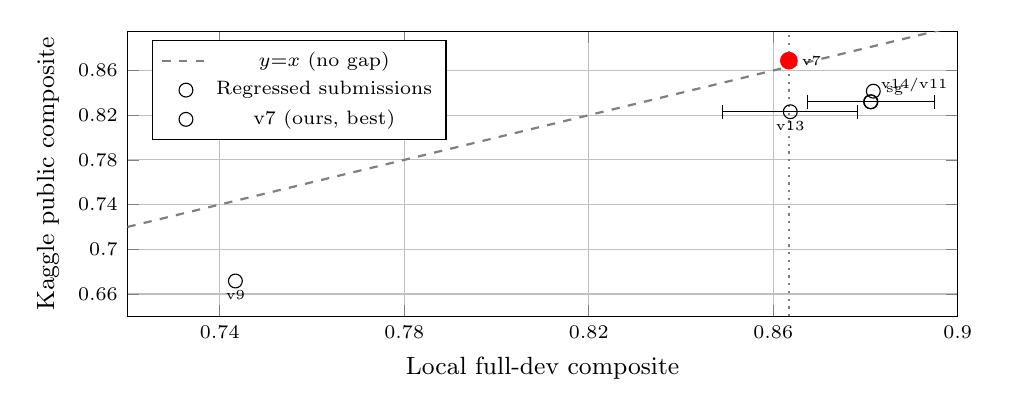
\begin{tikzpicture}
\begin{axis}[
  width=\columnwidth,
  height=52mm,
  xlabel={Local full-dev composite},
  ylabel={Kaggle public composite},
  xmin=0.720, xmax=0.900,
  ymin=0.640, ymax=0.895,
  xtick={0.74,0.78,0.82,0.86,0.90},
  ytick={0.66,0.70,0.74,0.78,0.82,0.86,0.90},
  tick label style={font=\scriptsize},
  label style={font=\small},
  grid=both,
  grid style={line width=0.2pt, draw=gray!30},
  major grid style={line width=0.4pt, draw=gray!50},
  legend style={font=\scriptsize, at={(0.03,0.97)}, anchor=north west},
]
% y=x reference line
\addplot[dashed, gray, thick, domain=0.72:0.90] {x};
\addlegendentry{$y{=}x$ (no gap)}

% Regressed submissions (hollow circles)
\addplot[only marks, mark=o, mark size=2.5pt, black]
  coordinates {
    (0.7434, 0.6716)   % v9
    (0.8811, 0.8320)   % v11 / DDL-v2
    (0.8817, 0.8415)   % struct-guard
  };
% v13 and v14 with 95% bootstrap CI error bars on x (local composite)
\addplot[only marks, mark=o, mark size=2.5pt, black,
  error bars/.cd, x dir=both, x explicit]
  coordinates {
    (0.8637, 0.8231) +- (0.0146, 0)   % v13: CI half-width=(0.014+0.015)/2; CI crosses v7 ref
    (0.8812, 0.8320) +- (0.0137, 0)   % v14: CI half-width=(0.032-0.004)/2; CI above v7 yet regressed
  };
\addlegendentry{Regressed submissions}
% Vertical reference line at v7 local score
\addplot[dotted, gray, thick, domain=0.640:0.895] coordinates {(0.8634,0.640)(0.8634,0.895)};

% v7 anchor (filled red)
\addplot[only marks, mark=*, mark size=3pt,
         mark options={fill=red, draw=red}]
  coordinates { (0.8634, 0.8688) };
\addlegendentry{v7 (ours, best)}

% Labels for key points
\node[font=\tiny, anchor=west] at (axis cs:0.8634,0.8688) {\,v7};
\node[font=\tiny, anchor=north] at (axis cs:0.7434,0.6716) {v9};
\node[font=\tiny, anchor=north] at (axis cs:0.8637,0.8231) {v13};
\node[font=\tiny, anchor=south west] at (axis cs:0.8812,0.8320) {v14/v11};
\node[font=\tiny, anchor=west] at (axis cs:0.8817,0.8415) {\,sg};
\end{axis}
\end{tikzpicture}
\caption{Local full-dev vs.\ Kaggle public composite. sg\,=\,structure-guard (\S\ref{sec:gap}). Diagonal: $y{=}x$ (no gap). Only v7 lies above it; all locally improved systems regressed. Horizontal bars on v13 and v14 show 95\% bootstrap CI for local composite; v13's interval overlaps the v7 reference (dotted vertical), confirming it was never a decisive offline win.}
\label{fig:gap}
\end{figure}

\begin{table}[t]
\centering
\resizebox{\columnwidth}{!}{%
\begin{tabular}{llccc}
\toprule
\textbf{Ver.} & \textbf{Key change} & \textbf{Local} & \textbf{Public} & \textbf{Private} \\
\midrule
v5 & Early pipeline & --- & 0.8043 & 0.8124 \\
v6 & Reranker added & --- & 0.8618 & 0.8517 \\
\textbf{v7} & \textbf{Cons.\ rollback} & \textbf{.8634} & \textbf{.8688} & \textbf{.8722} \\
v9 & Doc-level rerank & --- & 0.6716 & 0.7265 \\
struct.\ guard & Structure chunks & .8817 & 0.8415 & 0.8600 \\
v14 (DDL v3) & Dense-doc-lock & .8812 & 0.8320 & 0.8396 \\
v13 (refocus) & Prompt refocus & .8637 & 0.8231 & 0.8441 \\
\bottomrule
\end{tabular}%
}
\caption{Submission lineage. \textbf{v7} is the final best. All systems with positive local deltas regressed on Kaggle (Figure~\ref{fig:gap}).}
\label{tab:lineage}
\end{table}

v7 is a conservative rollback from v6: v6 submitted the Qwen3-4B reranker at \texttt{max\_length}=1024, a confounded experiment where halving the context budget dominated any model-size benefit. v7 restored the 0.6B reranker at \texttt{max\_length}=2048 with a minimal direct prompt, trading the local gains of v6's experimental features for cross-split stability.

Every system with a positive local delta regressed on Kaggle (Figure~\ref{fig:gap}, Table~\ref{tab:lineage}). Three patterns predict failure:

\textbf{(1) High doc flip rate.} v13 and v14 have doc flip rates of 6.3--6.9\% vs.\ 0\% for v7. Document changes without proportional accuracy gain indicate fragile routing that breaks under distribution shift.

\textbf{(2) Per-domain imbalance.} v13 gains on Domain 2 ($+$0.012) but loses on Domain 1 ($-$0.016). A domain-unbalanced local win is unreliable when the private test contains an unseen third domain.

\textbf{(3) Long-document proxy dependence.} Dense-doc-lock and structure-guard\footnote{Structure-guard: structure-aware chunking with document-level gating, abbreviated \textsc{sg} in Figure~\ref{fig:gap}.} candidates show stronger local gains on Domain 1 (long docs, avg.\ 78 pages) than Domain 2, creating selection bias toward heuristics tuned for the visible long-document distribution. A confidence-margin heuristic (\textsc{dense-margin-lock}: lock to top doc when retrieval margin $>$0.25) proved near-neutral across all evaluation splits (exactly tied on the three CV/lockbox splits, $-$0.002 on full-dev).

These three signals collectively suggest Domain 3 resembles Domain 2 (short documents, avg.\ 8.5 pp/doc) rather than Domain 1 (avg.\ 78.6 pp/doc): DDL and structure-guard, designed for long-doc retrieval where wrong-page distance spans 7+ pages (Domain 1 median), provide no benefit — and incur routing fragility — on short documents where within-1-page retrieval already dominates (Domain 2 median: 1 page). We cannot confirm this without access to private test documents, but all locally-improved systems targeting long-document properties failed on the private leaderboard.

\begin{table}[t]
\centering
\resizebox{\columnwidth}{!}{%
\begin{tabular}{lcccc}
\toprule
\textbf{System} & \textbf{Flip\%} & \textbf{Imbal.} & \textbf{Long-doc} & \textbf{Kaggle $\Delta$} \\
\midrule
v7 (ref.) & 0.0\% & No & No & $+$0.005 \\
v13 & 6.3\% & Yes & No & $-$0.046 \\
v14 & 6.9\% & Yes & Yes & $-$0.037 \\
struct.\ guard & 7.4\% & No & Yes & $-$0.027 \\
v9 & 30.2\% & Yes & No & $-$0.197 \\
\bottomrule
\end{tabular}%
}
\caption{Risk signals vs.\ Kaggle public outcome. ``Flip\%'' = doc change rate vs.\ v7 (full-dev). ``Imbal.'' = per-domain $\Delta{>}0.01$. ``Long-doc'' = heuristic targeting docs $\geq$25 pages. All four regressed systems showed $\geq$1 high-risk signal; v7 showed none.}
\label{tab:risk}
\end{table}

Table~\ref{tab:risk} formalizes these signals. A system passes the risk filter only if flip rate $<$5\%, no per-domain delta exceeds 0.01, and no long-document heuristic is active. All four post-v7 Kaggle-tested systems violated at least one criterion; v7 violated none, suggesting this as a practical pre-submission gate for future entries.

The v9 regression (0.6716 public) resulted from bundling six simultaneous changes; the majority of regressions followed the doc-level rerank change, illustrating the danger of compound commits.

\textbf{False-positive detection.} Our three-split gating caught \texttt{no\_bleed\_v1} before submission: fold-0 gain was $+$0.027 (the strongest offline win observed), yet fold-1 showed $-$0.010 and lockbox $-$0.030. The fold-0 win reflected noise amplification on 73 questions, not a robust improvement. Without multi-split gating, this would have been submitted.

\section{Error Analysis}
\label{sec:error}

\begin{table}[t]
\centering
\small
\begin{tabular}{lcc}
\toprule
\textbf{Category} & \textbf{N} & \textbf{\%} \\
\midrule
All correct (answer + doc + page) & 205 & 44.5 \\
Correct answer, right doc, wrong page & 169 & 36.7 \\
Wrong answer, right doc, wrong page & 39 & 8.5 \\
Correct answer, wrong doc & 21 & 4.6 \\
Wrong answer, right page & 17 & 3.7 \\
Wrong answer, wrong doc & 10 & 2.2 \\
\bottomrule
\end{tabular}
\caption{Error breakdown for v7 on full dev ($N$=461).}
\label{tab:errors}
\end{table}

The dominant error (36.7\%) is \textit{correct answer with wrong page}: BGE-M3 found the right document but ranked the wrong page first, yet MamayLM answered correctly because the true answer appeared in the 2-page context window.
Of the 169 wrong-page cases, \textbf{55.8\% are within 3 pages} of the true answer (median distance = 2 pages), confirming these are near-miss retrieval errors rather than retrieval failures.
The 37-point gap between page accuracy (48.2\%) and answer accuracy (88.5\%) demonstrates that multi-page context provides substantial resilience to page-level retrieval errors.

True retrieval failures (wrong document) account for only 6.8\% of questions, consistent with BGE-M3's Doc@1 = 0.933.
Domain 1 (long docs): Doc@1 = 0.975 but Page@1 = 0.409 --- exact page retrieval over 78-page documents is the binding bottleneck.
Domain 2 (short docs): Doc@1 = 0.901, Page@1 = 0.536.

Page localization difficulty differs sharply: Domain 1 wrong-page cases have \textbf{median distance 7 pages} (within-3-pages: 40\%), while Domain 2 has \textbf{median distance 1 page} (within-3-pages: 76\%). This explains why long-document heuristics showed larger local gains on Domain 1 --- they target a distributional property (deep page retrieval in 78-page documents) that is absent from the hidden Domain 3.

\section{Conclusion}

We presented PFW, a BGE-M3 + cross-encoder + MamayLM RAG pipeline achieving rank 7/15 (private 0.8722) at UNLP 2026. Our main finding is that conservative baselines beat local optimization under hidden domain shift: all offline improvements regressed on Kaggle. The clearest path to improvement is the fair 4B reranker ($+$0.023 composite, CI entirely positive) and reducing the page-proximity bottleneck that accounts for 36.7\% of errors. The per-domain page-distance analysis (\S\ref{sec:error}) suggests that page localization for long-document collections requires retrieval improvements that are robust to domain shift, not heuristics tuned to the visible document distribution.

\section*{Limitations}

All offline ablations use two visible domains; the hidden third private domain drives the local-vs-Kaggle gap and is not directly analyzable. Q4\_K\_M quantization of MamayLM reduces reasoning coherence — evidenced by CoT collapse to $\approx$14.3\% accuracy and consistent with quantization's documented effect on multi-step reasoning~\cite{dettmers2024qlora}; full-precision inference was infeasible within the 24~GB VRAM budget when co-loaded with the reranker. The 4B reranker, while showing robust offline improvement, could not be submitted within the 9-hour competition deadline on T4$\times$2 hardware.

\section*{Ethics Statement and Reproducibility}

MamayLM and BGE-M3 training data may contain societal biases, and domain-specific biases may affect performance on the hidden domain. All code, pipeline preset files (\texttt{pipeline\_presets.json}: 34 configurations), and per-question predictions for all offline benchmark runs are released at \url{https://github.com/Taleef7/UNLP-2026}. MamayLM and BGE-M3 weights are publicly available. This work complies with the ACL reproducibility checklist.

\bibliography{unlp2026}

\end{document}
